\documentclass[12pt]{article}
\usepackage{amsmath}
\usepackage{amssymb}
\usepackage[letterpaper,margin=0.85in,centering]{geometry}
\usepackage{fancyhdr}
\usepackage{enumerate}
\usepackage{lastpage}
\usepackage{multicol}
\usepackage{graphicx}

\reversemarginpar

\pagestyle{fancy}
\cfoot{Page \thepage \ of \pageref{LastPage}}\rfoot{{\bf Total Points: 40}}
\chead{MATH 1010A}\lhead{Test \# 2 MAKEUP}\rhead{Thursday, 19\textsuperscript{th} November, 2015}

\newcommand{\points}[1]{\marginpar{\hspace{24pt}[#1]}}
\newcommand{\skipline}{\vspace{12pt}}
%\renewcommand{\headrulewidth}{0in}
\headheight 30pt

\newcommand{\di}{\displaystyle}
\newcommand{\R}{\mathbb{R}}
\newcommand{\aaa}{\mathbf{a}}
\newcommand{\bbb}{\mathbf{b}}
\newcommand{\ccc}{\mathbf{c}}
\newcommand{\dotp}{\boldsymbol{\cdot}}
\newcommand{\abs}[1]{\lvert #1\rvert}
\newcommand{\len}[1]{\lVert #1\rVert}
\newcommand{\ivec}{\,\boldsymbol{\hat{\imath}}}
\newcommand{\jvec}{\,\boldsymbol{\hat{\jmath}}}
\newcommand{\kvec}{\,\boldsymbol{\hat{k}}}
\DeclareMathOperator{\comp}{comp}

\begin{document}

\author{Instructor: Sean Fitzpatrick}
\thispagestyle{plain}
\begin{center}
\emph{University of Lethbridge}\\
Department of Mathematics and Computer Science\\
19\textsuperscript{th} November, 2015, 10:00 - 10:50 am\\
{\bf MATH 1010A - Test \#2 Alternate}\\
\end{center}
\skipline \skipline \skipline \noindent \skipline
Last Name:\underline{\hspace{353pt}}\\
\skipline
First Name:\underline{\hspace{350pt}}\\
\skipline
Student Number:\underline{\hspace{323pt}}\\
\skipline
Tutorial Section: \underline{\hspace{320pt}}\\


\vspace{0.5in}


\begin{quote}
 {\bf Record your answers below each question in the space provided.    Left-hand pages may be used as scrap paper for rough work.  If you want any work on the left-hand pages to be graded, please indicate so on the right-hand page.
 
 \bigskip
 
Partial credit will be awarded for partially correct work, so be sure to show your work, and include all necessary justifications needed to support your arguments.

\bigskip

No external aids are allowed, with the exception of a 5-function calculator.}
\end{quote}


\vspace{0.5in}

For grader's use only:

\begin{table}[hbt]
\begin{center}
\begin{tabular}{|l|r|} \hline
Problem &Grade\\
\hline \hline
\cline{1-2} 1 & \enspace\enspace\enspace\enspace\enspace\enspace/8\\
\cline{1-2} 2 & \enspace\enspace\enspace\enspace\enspace\enspace/12\\
\cline{1-2} 3 & \enspace\enspace\enspace\enspace\enspace\enspace/10\\
\cline{1-2} 4 & \enspace\enspace\enspace\enspace\enspace\enspace/10\\
\cline{1-2} Total & \enspace\enspace\enspace\enspace\enspace\enspace/40\\
\hline
\end{tabular}

\skipline

\skipline

\skipline

B
\end{center}
\end{table}
\newpage


\begin{enumerate}
\item Match the following functions with their graphs below: \points{8}
\begin{align*}
 f(x) &= x^2(x+1)(x-2)^2, &h(x) &= \dfrac{(x+2)(x-1)}{(x+1)(x-2)},\\
 g(x) &= \frac{1}{3}(x+2)(x-1)(x-3), &k(x) &= \dfrac{9-x^2}{x^2-4}
\end{align*}

\bigskip

\begin{multicols}{2}
 \begin{center}
  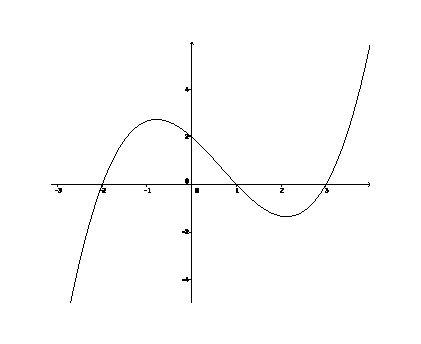
\includegraphics[width=3.25in]{poly1(b)}
 \end{center}

\bigskip

\bigskip

 \begin{center}
   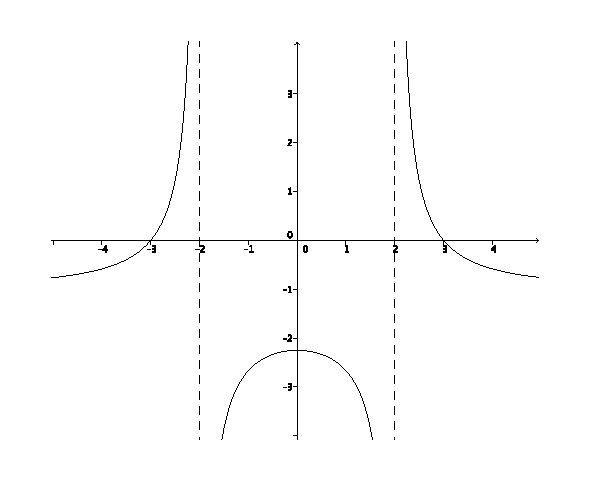
\includegraphics[width=3.25in]{rat1(d)}
 \end{center}
 \begin{center}
   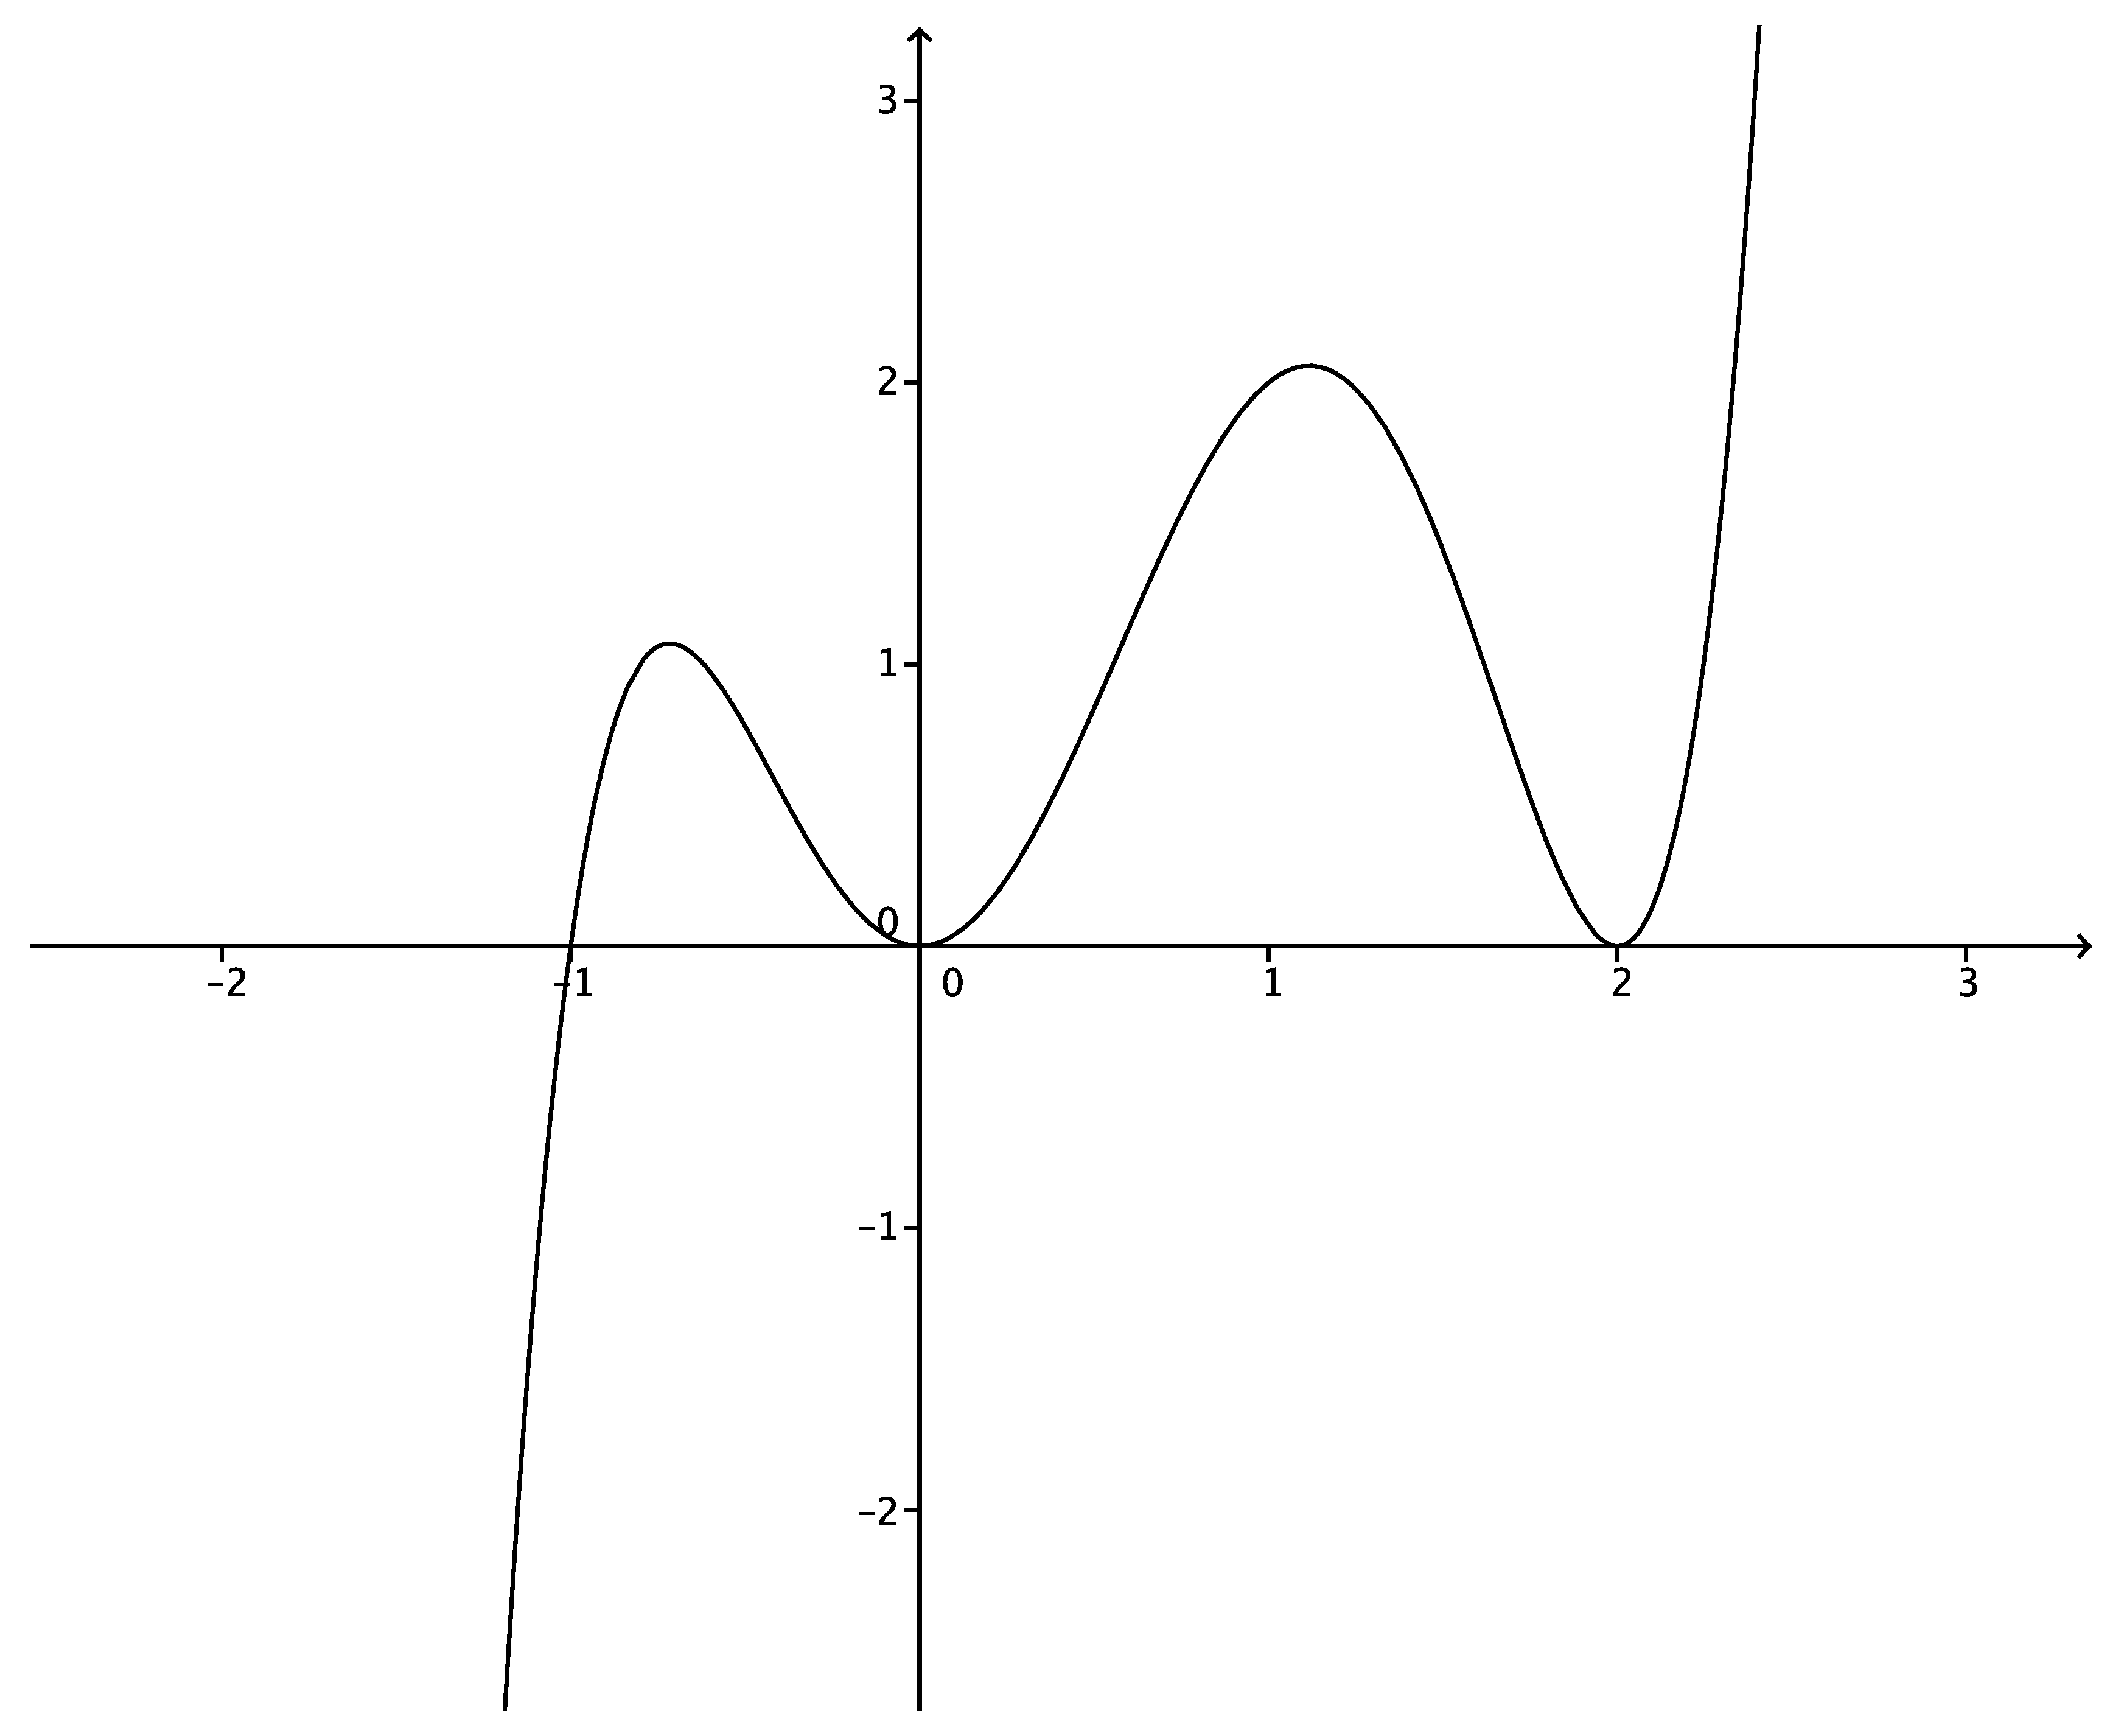
\includegraphics[width=3.25in]{poly1(d)}
 \end{center}

\bigskip

\bigskip

 \begin{center}
   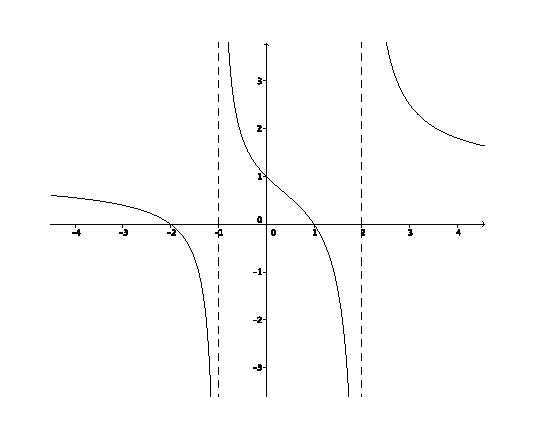
\includegraphics[width=3.25in]{rat1(a)}
 \end{center}
\end{multicols}


\newpage

\item Let $f(x) = x^3-3x^2-6x+8$.
\begin{enumerate}
 \item Show that $x-1$ is a factor of $f(x)$. \points{1}

\vspace{1in}

 \item Find $a,b\in\R$ such that $f(x) = (x-1)(x-a)(x-b)$. \points{4}

\vspace{3.5in}

 \item Construct the sign diagram for $f(x)$.  \points{2}

\vspace{1.5in}

 \item Solve the inequality $x^3+8\geq 3x^2+6x$. \points{2}

\newpage


 \item Sketch the graph of the function $f$ from the previous page. \points{3}
\end{enumerate}
\newpage

\item 
\begin{enumerate}
 \item Sketch the graph of $f(x) = \dfrac{x-1}{x^2+x}$. \points{6}

\vspace{4in}

 \item Solve the rational inequality $\dfrac{2}{x}-\dfrac{2}{x+1}\geq 1$. \points{4} 
\end{enumerate}

\newpage

\item \begin{enumerate}
       \item What are the values of $\sin\left(\dfrac{17\pi}{4}\right)$ and $\cos\left(\dfrac{-25\pi}{6}\right)$? \points{2}

\vspace{1.5in}

 \item What is the value of $\cos\left(\dfrac{5\pi}{12}\right)$? (Hint: $5=9-4$)\points{4}




 

%\item If $\cot\theta = \sqrt{5}$ with $\theta$ in Quadrant III, what is the value of $\sin\theta$? \points{3}

\vspace{3in}

\item Verify the identity $\dfrac{1}{1-\sin\theta} = \sec^2\theta+\sec\theta\tan\theta$. \points{4}
      \end{enumerate}


\end{enumerate}
\newpage

\begin{center}
 \textbf{Some stuff about trig functions that you possibly didn't remember}
\end{center}
\begin{itemize}
 \item Values of $\sin\theta$ and $\cos\theta$ in the first quadrant:
\begin{align*}
 \sin 0 &= 0  \quad& \quad \cos 0 &= 1\\
 \sin \pi/6 &= 1/2   \quad& \quad\cos \pi/6 &= \sqrt{3}/2\\
 \sin \pi/4 &= \sqrt{2}/2  \quad &\quad \cos \pi/4& = \sqrt{2}/2\\
 \sin \pi/3 &= \sqrt{3}/2   \quad &\quad\cos \pi/3& = 1/2\\
 \sin \pi/2 &= 1  \quad &\quad \cos \pi/2 &= 0
\end{align*}

\item Fundamental identities:
\begin{enumerate}
 \item $\tan\theta = \dfrac{\sin\theta}{\cos\theta}$, $\cot\theta = \dfrac{\cos\theta}{\sin\theta}$, $\sec\theta = \dfrac{1}{\cos\theta}$, $\csc\theta = \dfrac{1}{\sin\theta}$
 \item $\cos^2\theta + \sin^2\theta =1$
 \item $\cos(\alpha + \beta) = \cos\alpha\cos\beta - \sin\alpha\sin\beta$
 \item $\cos(\alpha - \beta) = \cos\alpha\cos\beta + \sin\alpha\sin\beta$
 \item $\sin(\alpha + \beta) = \sin\alpha\cos\beta + \cos\alpha\sin\beta$
 \item $\sin(\alpha - \beta) = \sin\alpha\cos\beta - \cos\alpha\sin\beta$
\end{enumerate}
\item Obvious but occasionally forgotten facts that are sometimes useful in conjunction with some of the identities above:
\begin{enumerate}
 \item $2\theta = \theta + \theta$
 \item $\theta = \dfrac{\theta}{2}+\dfrac{\theta}{2}$
\end{enumerate}


\end{itemize}


\end{document}